\chapter{Results}\label{chap:Results}

% Update?
In this chapter, the results of the analysis are presented. \textbf{Chapter \ref{sec:Exploratory_Data_Analysis}} provides an overview of the data and explores the fairness of the dataset. 
\textbf{Chapter \ref{sec:Results}} presents the results of the analysis. \textbf{Chapter \ref{sec:Limitations}} discusses the limitations of the analysis.

\section{Exploratory Data Analysis}\label{sec:Exploratory_Data_Analysis}



\subsection{Data Overview}\label{subsec:Data_Overview}

% Standard Dataset Metrics

% Histograms of numeric variables from V2 pipeline notebook 
% Maybe correlation matrix from V2 pipeline notebook
% Maybe distribution boxplots from V2 pipeline notebook

\subsection{Fairness}\label{subsec:Fairness}

% Probably rename - tie to Hypothesis and Research Questions

% Graph on grant by race, accompanied by additional information from NN notebook like difference in groups etc.

Potential unfairness in the underlying data can be identified from assessing the distribution of the target variable across different groups.
\textbf{Figure \ref{fig:CHXX_Loan_Grant_By_Protected_Attribute}} shows the amount of (not) granted loans per race and by sex, the probabilities of being granted a loan across these groups can be found in \textbf{Table \ref{tab:loan_granting}}.\@

\begin{figure}[h]
    \centering
    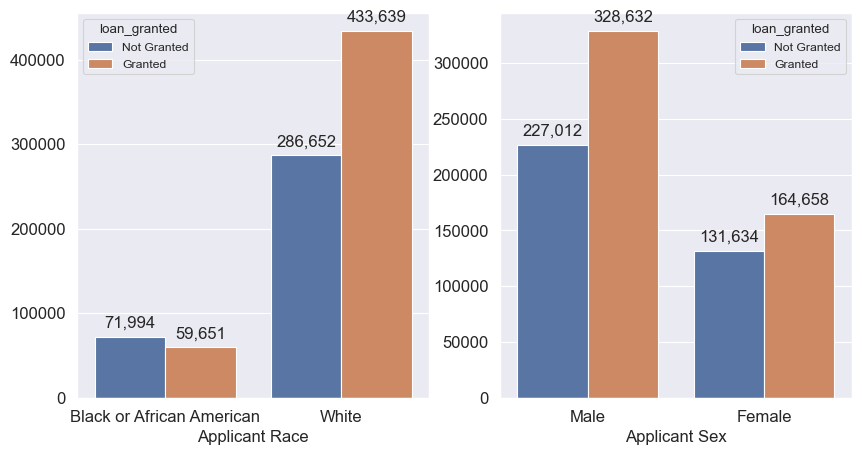
\includegraphics[width=0.85\textwidth]{CHXX_Loan_Grant_By_Protected_Attribute.png}
    \caption{Loan Grant by Protected Attribute}
    \label{fig:CHXX_Loan_Grant_By_Protected_Attribute}
\end{figure}

\begin{table}[htbp]
    \centering
      \begin{tabular}{lcc}
      \toprule
      \textbf{Applicant Race} & \textbf{Applicant Sex} & \textbf{Loan Granted (\%)} \\
      \midrule
      Black or African American & Male    & 46.4 \\
            & Female  & 44.1 \\
      White & Male    & 60.9 \\
            & Female  & 58.8 \\
      \bottomrule
      \end{tabular}%
      \caption{Loan Granting Statistics by Applicant Race and Sex}
    \label{tab:loan_granting}%
\end{table}%


\section{Results}\label{sec:Results}        



\section{Limitations}\label{sec:Limitations}